\documentclass{article}
\usepackage{graphicx}
\usepackage[margin=1.5cm]{geometry}
\usepackage{amsmath}

\begin{document}

\title{Tuesday Reading Assessment: Chapter 2-1 through 2-7}
\author{Prof. Jordan C. Hanson}

\maketitle

\begin{figure}[ht]
\centering
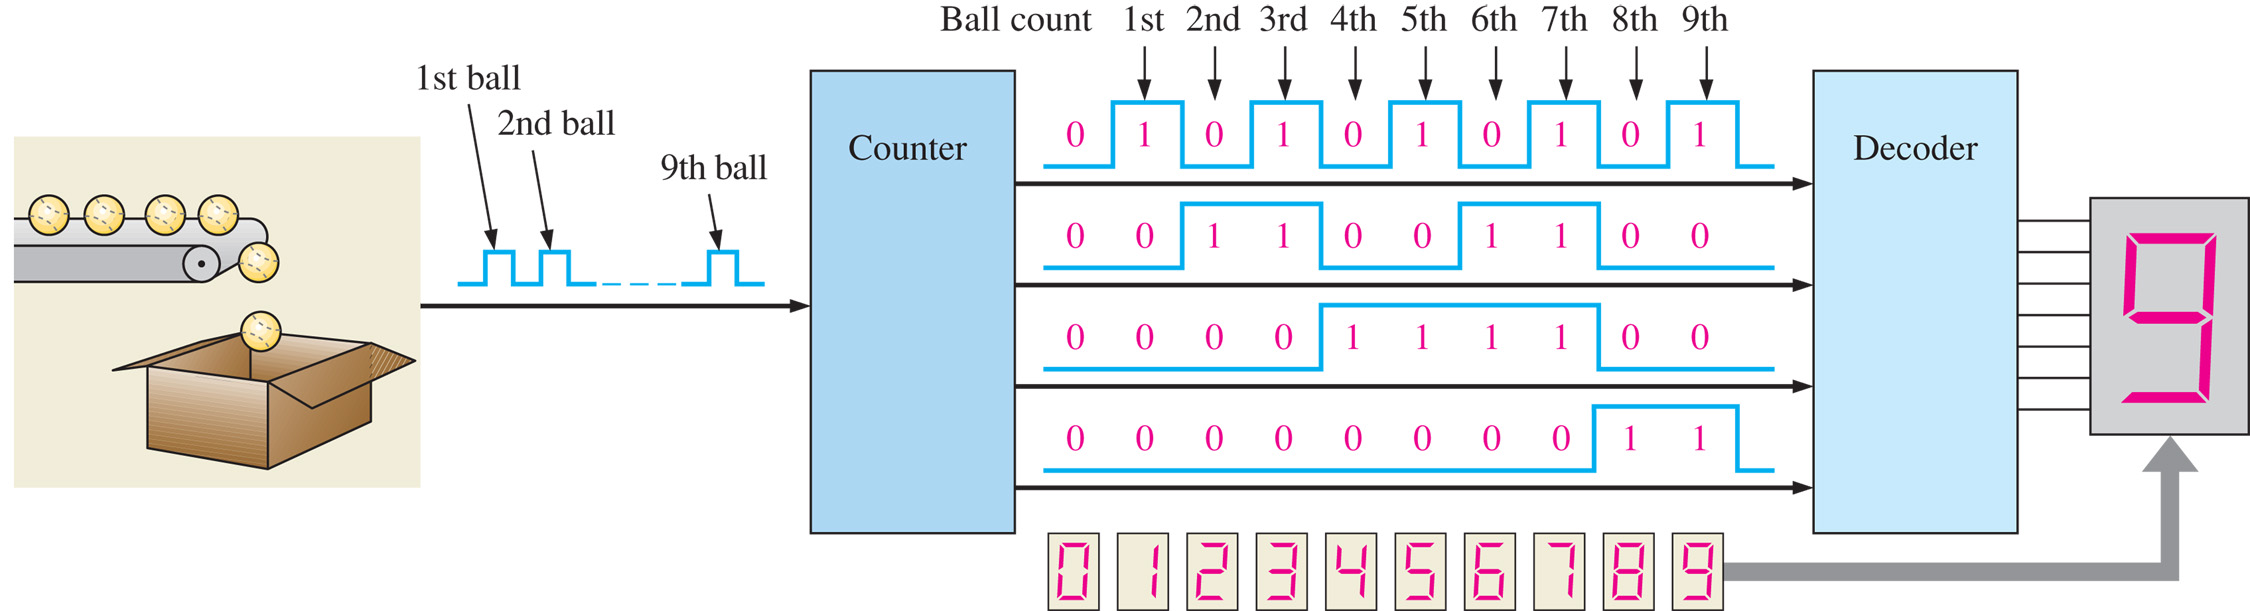
\includegraphics[width=0.65\textwidth]{figures/counter_balls.jpg} \\ \vspace{0.25cm}
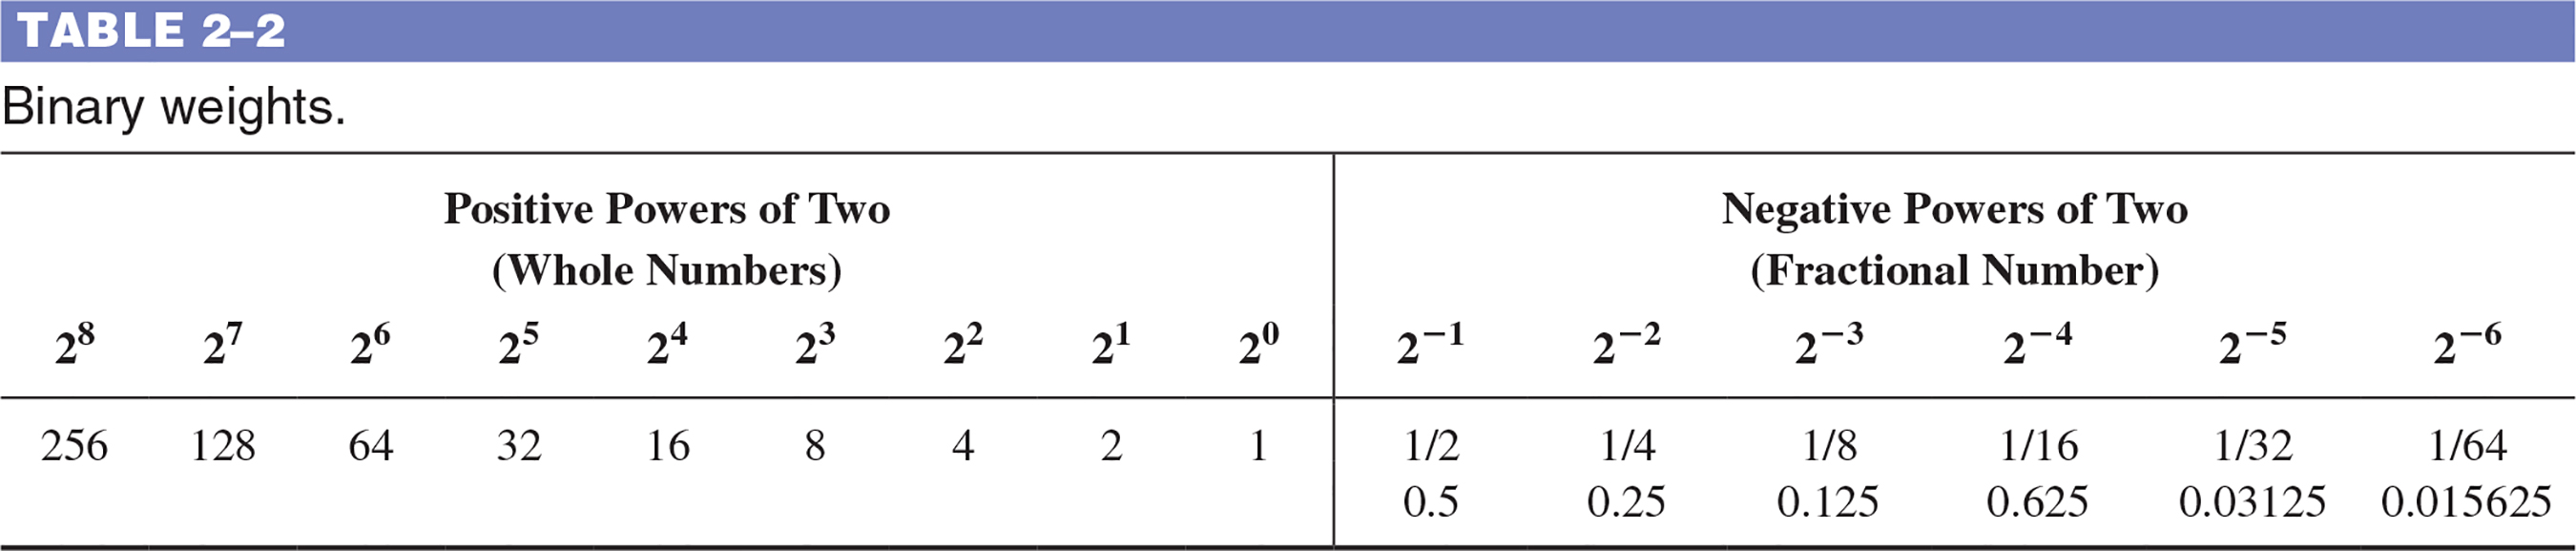
\includegraphics[width=0.65\textwidth]{figures/binary_weights.jpg}
\caption{\label{fig:quiz} (Top) A sensor provides digital pulses to a counter with four outputs. (Bottom) A conversion table for binary weights.}
\end{figure}

\section{Binary to Decimal, Decimal to Binary, 2's complement, Addition}

\begin{enumerate}
\item Considering Fig. \ref{fig:quiz} (bottom), convert the following binary numbers to decimal:
\begin{itemize}
\item 1000
\item 1010
\item 1011
\item 1111
\end{itemize}
\item Using repeated division by 2 method, convert the following decimal numbers to binary:
\begin{itemize}
\item 255
\item 44
\item 64
\item 31
\end{itemize}
\item What is the 2's complement of 125 in binary? \\ \vspace{0.5cm}
\item What is 1101 + 1011, assuming these are binary numbers? \\ \vspace{0.5cm}
\item If the counter in Fig. \ref{fig:quiz} (top) takes 18 seconds to reach 1001, how many seconds per count?
\end{enumerate}

\end{document}
